\chapter{Half-plane with Robin boundary} \label{chapter-robin}
In this chapter we will examine the Landau Hamiltonian of a particle confined to a half-plane with a Robin (or \textit{mixed}) boundary condition. Let $\alpha \in \R$ and $\Omega := \R \times \R_+$, where $\R_+ \equiv [0, +\infty)$, then the Hamiltonian is given by\footnote{
    The equalities are to be understood in the weak sense again. $(H_\alpha \psi)(x, y) = ...$ holds for almost every $(x,y)$ in $\Omega$ with respect to the Lebesgue measure. $\psi(0,y) \equiv \lim_{x \to 0} \psi(x,y) = ...$ holds for almost every $y\in\R$, and the limit is the \textit{essential} limit wrt. the Lebesgue measure.
}
\begin{equation}
    \begin{gathered}
        \big( H_\alpha \psi \big)(x,y)
        = \left(
            -\pd{^2}{x^2} +
            \big( \i \pd{^2}{y^2} + bx \big)^2
        \right) \, \psi(x,y) \: ,
        \\
        \Domain(H_\alpha)
        = \big\{ \,
            \psi \in W^{2,2}(\Omega) \cap L^2_{x^4}(\Omega)
            \; \big| \;
            \psi(0,y) + \alpha \, \psi'(0,y) = 0
        \, \big\} \: .
    \end{gathered}
\end{equation}
Using \eqref{eqn-vague-direct-integral-decomp}, we can once again show that the Hamiltonian is unitarily equivalent to a direct integral $H_\alpha = \int^\oplus_\R \Hf_\alpha(p) \d{p}$, where $\Hf(p)$ is the fiber Hamiltonian given by
\begin{equation}
    \begin{gathered}
        \big( \Hf_\alpha(p) \varphi \big)(x)
        = -\varphi''(x) + (p + bx)^2 \, \varphi(x) \: ,
        \\
        \Domain( \Hf_\alpha(p) )
        = \big\{ \,
            \varphi \in W^{2,2}(\R_+) \cap L^2_{x^4}(\R_+)
            \; \big| \;
            \varphi(0) + \alpha \, \varphi'(0) = 0
        \, \big\} \: .
    \end{gathered}
\end{equation}

\section{Well-posedness}
We will start by showing that the Hamiltonian is bounded from below, starting with the fibre Hamiltonian:
\begin{align*}
    \\[-2\baselineskip]
    &\big( \varphi, \Hf_\alpha(p) \, \varphi \big)
    = - \int_{\R_+} \overline\varphi \varphi''
    + \overbrace{\int_{\R_+} (bx + p)^2 \, |\varphi|^2}^{\geq 0}
    \geq -\big[ \overline\varphi \varphi' \big]_0^{\infty}
    + \int_{\R_+} |\varphi'|^2
    = \\ &\qquad
    = \overline{ \varphi(0) } \, \varphi'(0)
    + \norm{ \varphi' }_{L^2(\R_+)}^2
    = - \frac{1}{\alpha} \, \big| \varphi(0) \big|^2
    + \norm{ \varphi' }_{L^2(\R_+)}^2
    \: .
\end{align*}
We have used integration by parts, the fact that for $\varphi \in W^{2,2}$ both $\varphi$ and $\varphi'$ vanish at infinity, and finally the boundary condition $\alpha \, \varphi'(0) = -\varphi(0)$. For~$\alpha < 0$, the whole right-hand side is non-negative, hence we have found the lower bound. For~$\alpha > 0$, we have:
\begin{align*}
    &\big( \varphi, \Hf_\alpha(p) \, \varphi \big)
    \geq - \frac{1}{\alpha} \, \big| \varphi(0) \big|^2
    + \norm{ \varphi' }_{L^2(\R_+)}^2
    \geq -\frac{1}{\alpha} \norm{\varphi}_{L^{\!\infty}(\R_+\!)}
    \! + \norm{ \varphi' }_{L^2(\R_+\!)}^2
    \: .
\end{align*}
Now using the lemma \ref{lemma-sobolev-type-inequality} from the Appendix, we know that for every $a>0$ there exists $b>0$ such that $-\frac{1}{\alpha} \norm{\varphi}_{L^{\!\infty}} \geq -\frac{a}{\alpha} \norm{\varphi'}_{L^2} - \frac{b}{\alpha} \norm{\varphi}_{L^2}$. Setting $a = \alpha$, we obtain
\begin{equation*}
    \big( \varphi, \Hf_\alpha(p) \big)
    \geq
    \big( 1 - \frac{b}{\alpha} \big) \,
    \norm{\varphi}_{L^2(\R_+)}
    \: .
\end{equation*}
As demonstrated in \eqref{eqn-fiber-hamiltonian-lower-bound} in the previous chapter, the Hamiltonian $H$ is therefore also bounded from below with the same lower bound.

Now we will show the self-adjointness, again starting with the fibre Hamiltonian. Let $\varphi \in \Domain(\Hf_\alpha(p))$ and $\psi \in M \subset L^2(\R_+\!)$.
\begin{align*}
    \big(\Hf_\alpha(p) \, \varphi, \; \psi \big)
    &= \int_{\R_+}\!\! -\overline\varphi'' \psi + \int_{\R_+}\!\! \big(bx + p\big)^2 \, \overline\varphi \, \psi \\
    &= - \big[ \overline\varphi' \, \psi \big]_0^\infty
    + \big[ \overline\varphi \, \psi' \big]_0^\infty
    + \int_{\R_+}\!\! -\overline\varphi \, \psi'' + \int_{\R_+}\!\! \big(bx + p\big)^2 \, \overline\varphi \, \psi \\
    &= \underbrace{
        - \overline\varphi'(0) \, \psi(0)
        + \overline\varphi(0) \, \psi'(0)
        \vphantom{\Big|}
    }_{
        -\overline\varphi'(0) \,
        \big( \psi(0) + \alpha \psi'(0) \big)
    }
    + \int_{\R_+}\!\! \overline\varphi \, \big( {-\psi''} + (bx+p)^2 \psi \big) \: .
\end{align*}
First, we integrated by parts, assuming that $M\subseteq W^{2,2}(\R_+\!)$ ­– if it weren't, the result couldn't be independent of $\varphi$, as demonstrated in the previous chapter after \eqref{eqn-dirac-fiber-selfadj}. Then we used the fact that functions from $W^{2,2}$ vanish at infinity, and finally we applied the boundary condition $\varphi'(0) + \alpha \varphi'(0) = 0$. It is clear that $\psi$ must fulfill the same boundary condition in order for the result to be independent of $\varphi'(0)$. Therefore $M=\Domain(\Hf_\alpha(p))$ and the fibre Hamiltonian is self-adjoint. The Hamiltonian $H$, a direct integral of a self-adjoint operator, is hence also self-adjoint.

Lastly, we will show that the spetrum of $\Hf_\alpha(p)$ is discrete using the theorem~\ref{thm-sym-extension-spectrum}. We define:
\begin{equation*}
    \Omega = \big\{ \varphi \in W^{2,2}(\R_+\!) \cap L^2_{x^4}(\R_+\!) \;\big|\; \varphi(0) = \varphi'(0) = 0 \big\}
    \: ,
\end{equation*}
then the fibre Hamiltonians for all values of $\alpha$ have a common symmetric restriction:
\begin{equation*}
    h(p) := \Hf_\alpha(p) |_\Omega
\end{equation*}
\textbf{[Finish this section: show $h$ is closed and $n_+=n_-<\infty$.]}

\section{Eigenproblem of the fiber Hamiltonian}
We are searching for a function $\epsilon(p)$, such that for every $p$ there exists a $\varphi \in \Domain(\Hf_\alpha(p))$ for which
\begin{align*}
    \Hf_\alpha(p) \, \varphi = \epsilon(p) \, \varphi
    \: .
\end{align*}
Substituting from the definition, we get
\begin{align*}
    -\varphi''(x) + (p + bx)^2 \, \varphi(x)
    &= \epsilon \, \varphi(x)
    \: , \\
    \big( (p + bx)^2 - \epsilon \big) \, \varphi(x)
    &= \varphi''(x)
\end{align*}
This is the parabolic cylinder equation and, as in the previous chapter, its solutions are in the form
\begin{equation*}
    \varphi(x) = c \, D_\nu(w) + d \, D_\nu(-w)
    \: ,
    \quad \text{where} \quad
    w := \sqrt{2b} \big( x + \frac{p}{b} \big)
    \: , \quad
    \nu := \frac{\epsilon - b}{2b}
    \: .
\end{equation*}
Except for $\nu\in\N$, the $D_\nu(-w)$ term diverges exponentially, therefore $d$ must be zero in order for $\varphi\in\Domain(\Hf_\alpha)$. Now we apply the boundary condition:
\begin{align*}
    \varphi(0) &= \alpha \, \varphi'(0)
    \: ,
    \\[5pt]
    c \, D_\nu(w_0)
    &= \alpha \, \dd{}{x} \, c  D_\nu(w_0)
    \: ,
    \quad \text{where} \quad
    w_0 = \sqrt{2b} \, (0 + \tfrac{p}{b}) = p \, \sqrt{\tfrac{2}{b}}
    \: ,
    \\[5pt]
    D_\nu(w_0)
    &= \frac{\alpha}{\!\!\sqrt{2b}} \big(
        \frac{w_0}{2} D_\nu(w_0)
        - D_{\nu+1}(w_0)
    \big)
    \: ,
    \\[5pt]
    D_{\nu+1}(w_0)
    &=
    \big( 1 - \tfrac{\sqrt{2b}}{\alpha} \big)
    \frac{w_0}{2} D_\nu(w_0)
    \: ,
    \\[5pt]
    D_{\nu+1}(p \, \sqrt{\tfrac{2}{b}})
    &=
    \big( \tfrac{1}{\sqrt{2b}} - \tfrac{1}{\alpha} \big)
    \, p \, D_\nu(p \, \sqrt{\tfrac{2}{b}})
    \: .
    \numberthis\label{eqn-robin-spectral}
\end{align*}
The equation \eqref{eqn-robin-spectral} is the spectral condition, it defines the implicit function $\nu(\alpha)$, which in turn tells us, which values of $\epsilon$ are in the spectrum of $\Hf_\alpha$.

\textbf{[Grafy následují na další stránce.]}




\begin{figure}[p]
    \centering
    \noindent
    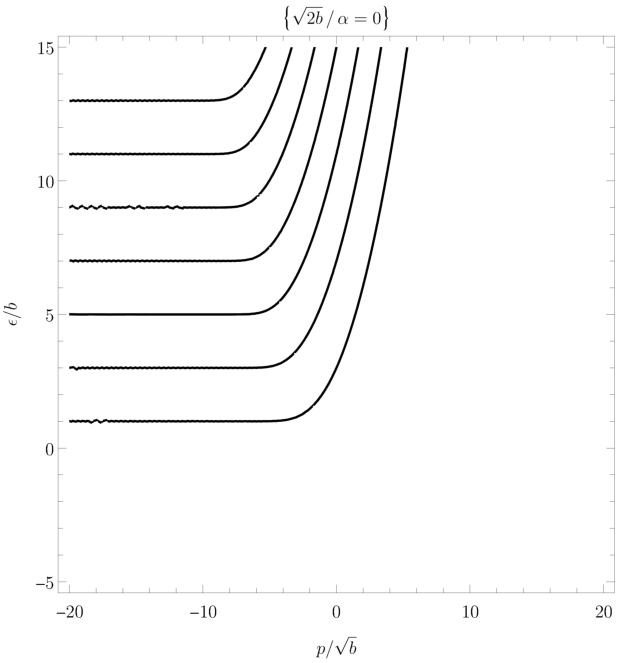
\includegraphics[width=0.45\textwidth]{grafy/robin0.pdf}%
    \hspace{0.1\textwidth}%
    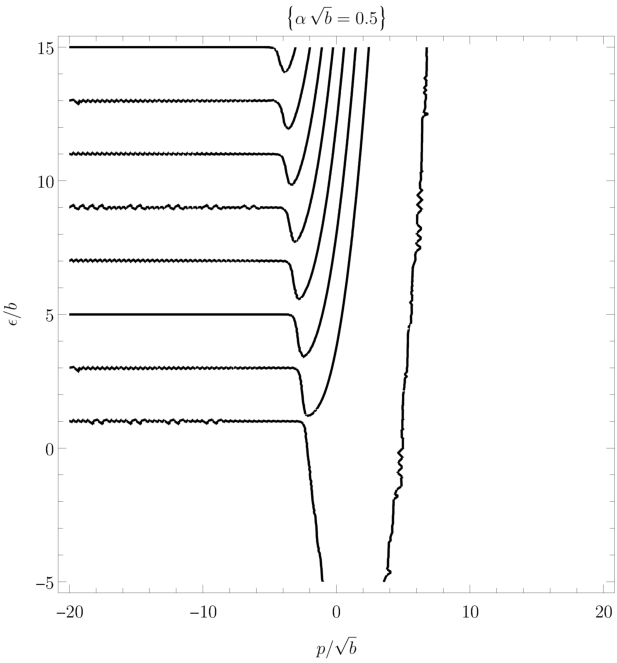
\includegraphics[width=0.45\textwidth]{grafy/robin0.5.pdf}%
    \\[1em]%
    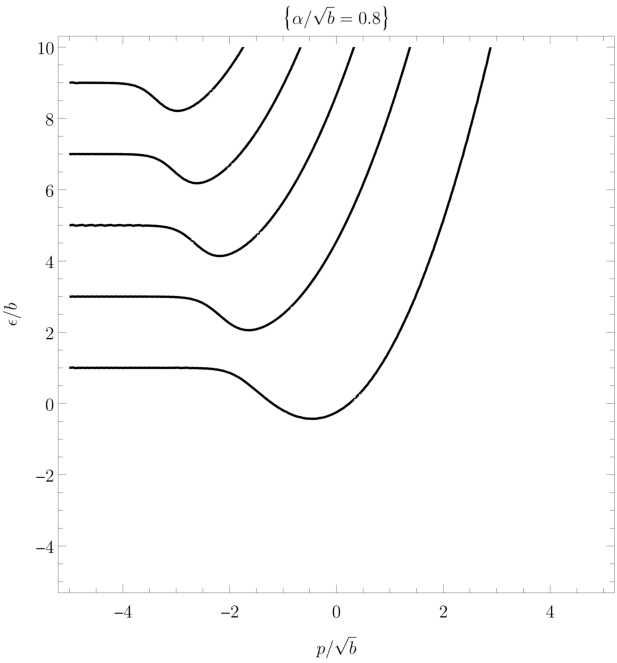
\includegraphics[width=0.45\textwidth]{grafy/robin0.8.pdf}%
    \hspace{0.1\textwidth}%
    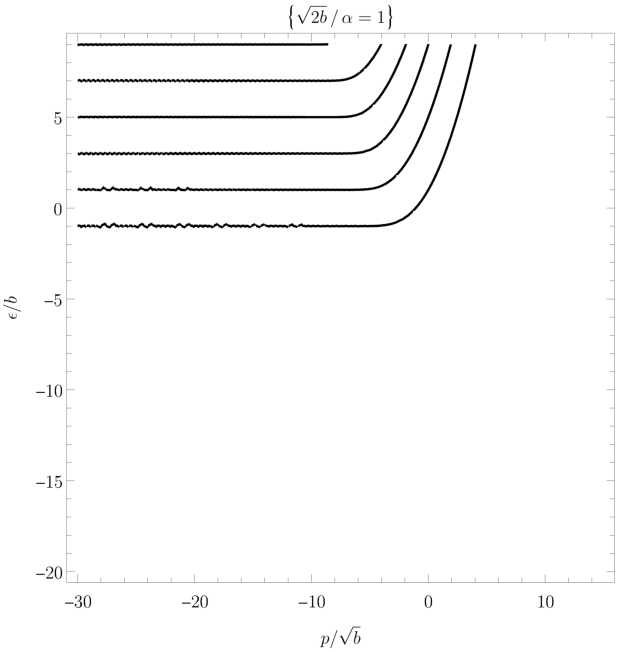
\includegraphics[width=0.45\textwidth]{grafy/robin1.pdf}%
    \\[1em]%
    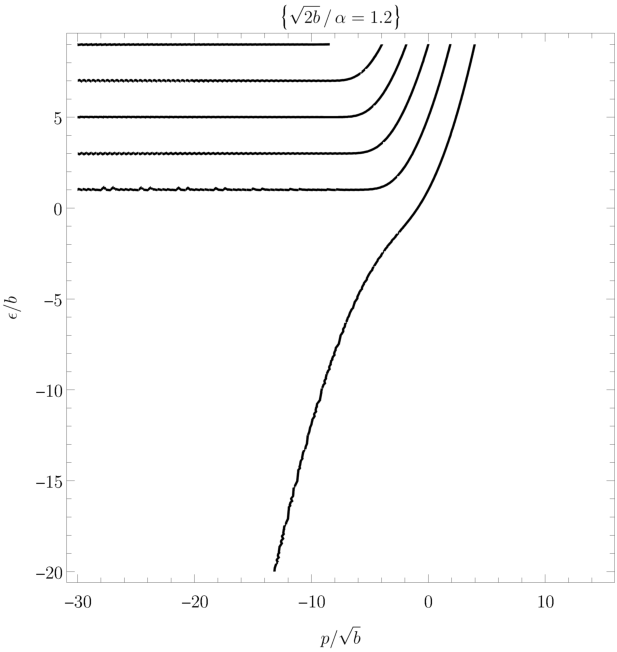
\includegraphics[width=0.45\textwidth]{grafy/robin1.2.pdf}%
    \hspace{0.1\textwidth}%
    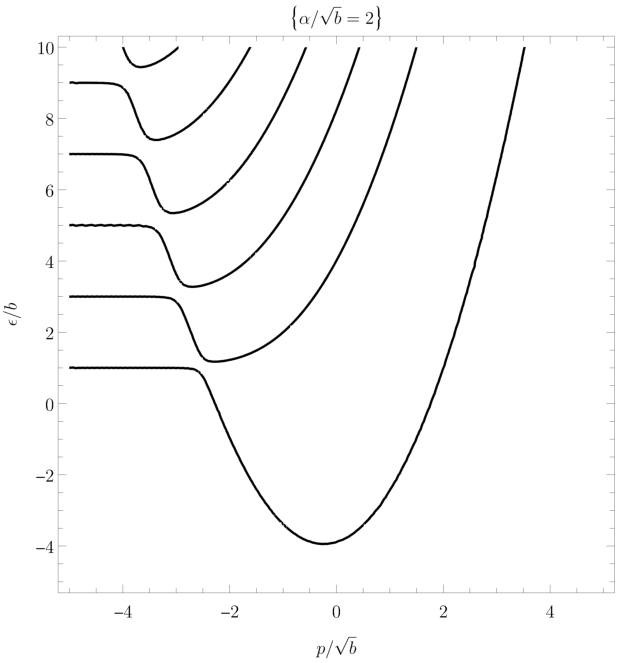
\includegraphics[width=0.45\textwidth]{grafy/robin2.pdf}\par
    \caption{The first energy levels $\epsilon$ as a function of the $y$-momentum $p$ for $\alpha\,\sqrt{2b} = 0.0, 0.5, 0.8, 1.0, 1.2$ and $2.0$ (starting with a system with Dirichlet bc.).}
    \label{plots-robin-positive}
\end{figure}

\begin{figure}[p]
    \centering
    \noindent
    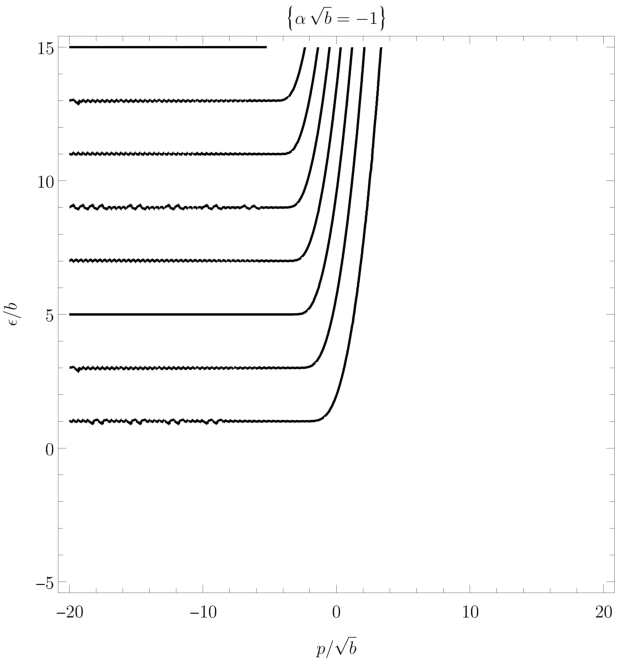
\includegraphics[width=0.45\textwidth]{grafy/robin-1.pdf}%
    \hspace{0.1\textwidth}%
    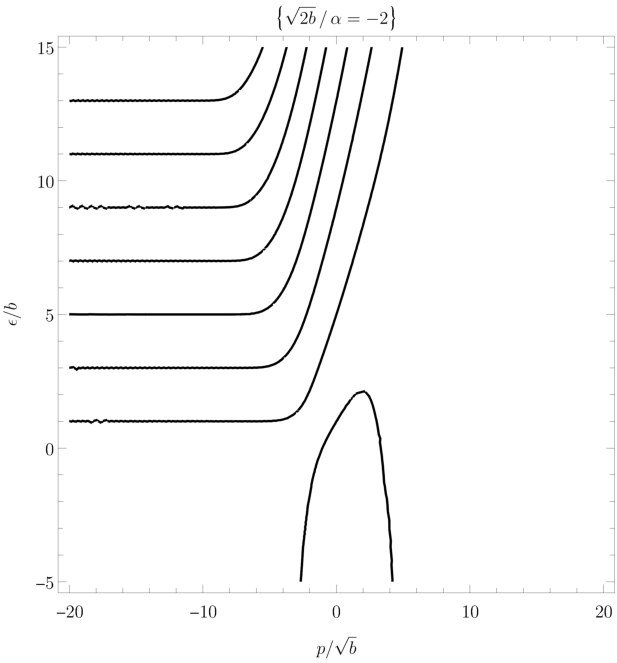
\includegraphics[width=0.45\textwidth]{grafy/robin-2.pdf}%
    \\[2em]%
    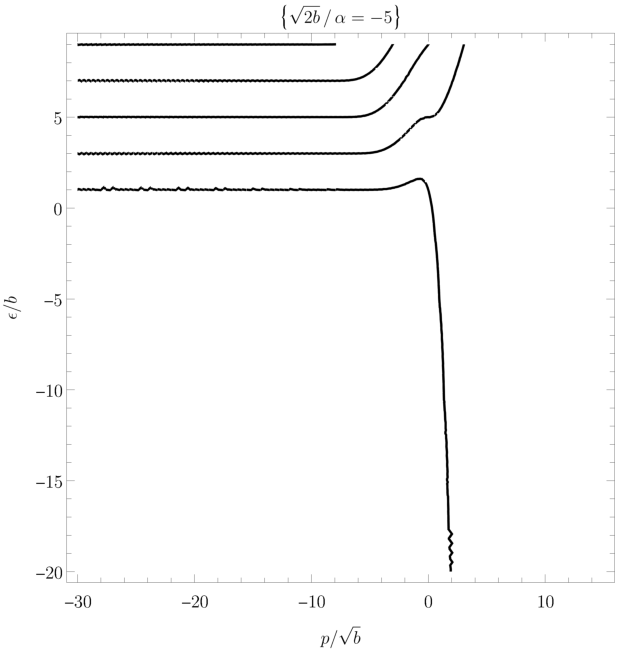
\includegraphics[width=0.45\textwidth]{grafy/robin-5.pdf}%
    \hspace{0.1\textwidth}%
    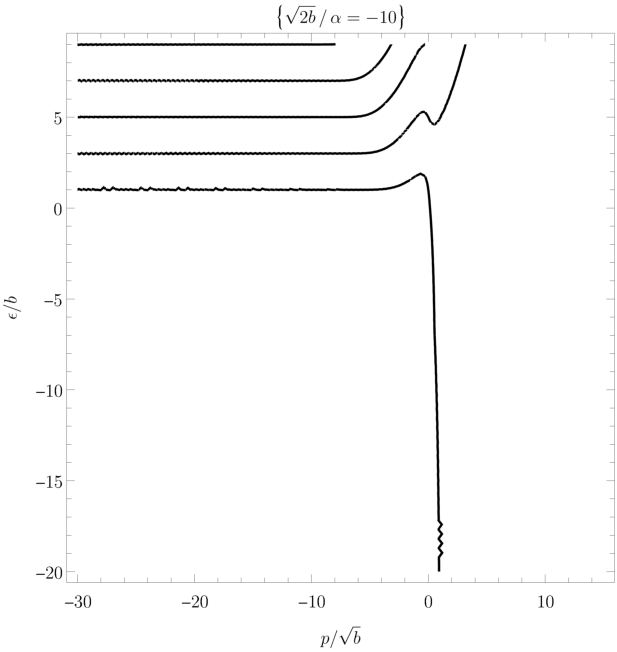
\includegraphics[width=0.45\textwidth]{grafy/robin-10.pdf}\par
    \caption{The first five energy levels $\epsilon$ as a function of the $y$-momentum $p$ for $\alpha\,\sqrt{2b} = -1, -2, -5$ and $-10$.}
    \label{plots-robin-negative}
\end{figure}
